\documentclass[a4paper,12pt]{scrartcl}
\usepackage[utf8]{inputenc}
%\usepackage[T1]{fontenc}
\usepackage[ngerman]{babel}
\usepackage[babel]{csquotes}
\usepackage{fancyhdr}
\usepackage{amssymb}
\usepackage[fleqn]{amsmath}
\usepackage[a4paper, left=30mm, right=25mm, bottom=25mm, top=30mm]{geometry}
\usepackage{tipa}
\usepackage{titlesec}
\usepackage{graphicx}
\usepackage[labelfont=bf]{caption}
\usepackage{subcaption}
\usepackage{float}
\usepackage{tocloft}
\usepackage{booktabs}
\usepackage{multirow}
\usepackage{multicol}
\usepackage{array}
\usepackage[exponent-product = \cdot]{siunitx}
\usepackage{cancel}
\sisetup{per-mode=fraction}

%\usepackage{pythontex}
\graphicspath{ {.} {img/} }

\usepackage[usenames, divpsnames]{xcolor}
\definecolor{footer-gray}{gray}{0.5}

\usepackage[textsize=scriptsize]{todonotes}

\title{Frequenzgangangalyse}
\date{2014-12-03}

\renewcommand{\cftsecdotsep}{\cftdotsep}

\pagestyle{fancy}
\linespread{1.3} % entspricht 1.5-fachem Zeilenabstand
\setlength{\parskip}{10pt}
\setlength{\parindent}{0mm}
\setlength{\mathindent}{10mm}

% enable draft mode --> revision is being shown
\newcount\draft\draft=1

\ifnum\draft=1
	\IfFileExists{revision.tex}{
		\include{revision}
	}{
		\newcommand{\Revision}{}
	}
\fi

\lhead{Frequenzganganalyse}
\chead{}
\rhead{\thepage}

\ifnum\draft=1
	\lfoot{\textcolor{footer-gray}{\today; rev. \Revision}}
\else
	\lfoot{}
\fi
\cfoot{}
\rfoot{}

% Page Numbering
%\setcounter{tocdepth}{3}
\usepackage{hyperref}
\hypersetup{
    colorlinks,
    citecolor=black,
    filecolor=black,
    linkcolor=black,
    urlcolor=black
}

%\newcommand{\todo}[1]{\textcolor{red}{TODO: #1}}

\usepackage[backend=biber, style=alphabetic-verb, sortlocale=de_DE, natbib=false, url=true, doi=true, eprint=true]{biblatex}
\addbibresource{sources.bib}

\begin{document}

\thispagestyle{empty}
\newgeometry{left=3cm, right=3cm}
\begin{center}
\vspace*{20mm}

\Large
\textbf{Grundpraktikum Maschinenlabor} \\
\vspace{10mm}
\Huge
\textbf{\textsf{Frequenzgangangalyse}} \\
\vspace{10mm}
\large
\textbf{\textsf{Praktikumsbericht}} \\
\textbf{\textsf{Mittwoch, 04. Dezember 2014}} \\
\textbf{\textsf{Gruppe 6}} \\
\ifnum\draft=1
	\textsf{\textcolor{footer-gray}{Version \textit{\Revision} vom \today}} \\
\fi

\vspace{40mm}
\begin{tabular}{rcl}
Ole Brinkmann & 406572 & obr11@tu-clausthal.de \\[4mm]
Lasse Fröhner & 420013 & lf12@tu-clausthal.de \\[4mm]
Sebastian Löhr & 341792 & swl@tu-clausthal.de \\[4mm]
Anna Stillfried & 421777 & apmsr12@tu-clausthal.de \\[4mm]
\end{tabular}

\end{center}

\pagebreak
\restoregeometry

\addtocontents{toc}{\protect\thispagestyle{fancy}}
\addtocontents{lof}{\protect\thispagestyle{fancy}}
\pagenumbering{Roman}
\tableofcontents
%\vspace{20mm}
%\listoffigures
%\vspace{20mm}
%\listoftables
\newpage

\pagenumbering{arabic}

\section{Einleitung}
Der sechste Versuch im Grundpraktikum Maschinenlabor WS 2014/15 vom 03.12.2014 am Institut für elektrische Informationstechnik befasst sich mit der Auswertung des Übertragungsverhalten eines dynamisch ermittelten Systems(Identifikation).

Die Übertragungsglieder lassen sich sowohl im Zeitbereich, wie auch im Frequenzbereich analysieren \cite{RegTech}.
Auf das dynamische System wird eine Eingangsgröße (Sinusfunktion) aufgegeben und eine Ausgangsgröße (Sinusantwort) mithilfe des Übertragungs\-verhalten des Übertragungsgliedes (LZI-Glied) ausgegeben.
Hierdurch werden Phasenverschiebung und Winkelauslenkung für beide Frequenzspektren aufgenommen und miteinander verglichen.
Das Oszilloskop zeigt die Sprungfunktion, sowie die Sinusfunktion.
Aus diesem Vergleich wird der Frequenzgang bei Aufschaltung eines harmonischen, sinusförmigen Eingangssignales für alle Frequenzen beschrieben.
Der Frequenzgang wird in Phasen und Amplitudengang aufgeteilt und in Form eines Bodediagramms graphisch dargestellt.
Die Analysen hierfür können zur Erstellung neuer schwingfähiger System wie auch zur Verbesserung bestehender Systeme dienlich sein.
Ziel dieser Frequenzganganalyse ist es den mathematischen Zusammenhang zwischen den Ein- und Ausgangsgrößen herzustellen, die Übertragungsfunktion.

\section{Aufbau}

\begin{figure}[h]
\centering
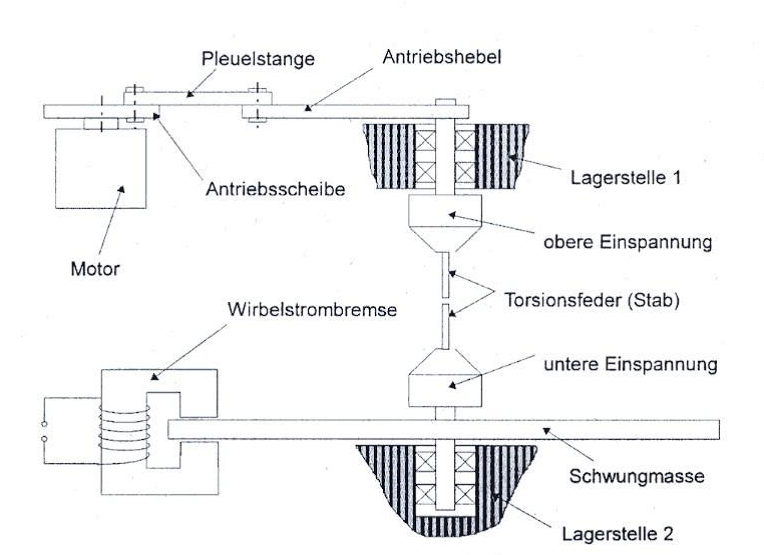
\includegraphics[width=\textwidth]{aufbau.png}
\caption{Versuchsaufbau nach \cite{skript}}
\label{fig:aufbau}
\end{figure}

Eine Frequenzganganalyse wird an einem Federpendel durchgeführt, bestehend aus einer Torsionsfeder und einer Schwungmasse.
Eine Wirbelstrombremse dient als Systemdämpfung. Die Wirbelstrombremse ist stufenlos einstellbar. Eine Spule erzeugt ein elektromagnetisches
Feld in der Aluminiumschwungscheibe. Es entsteht ein kreisförmiger Stromfluss bzw. ein Wirbelstrom aufgrund der Lorentzkraft.
Der Wirbelstrom hat ein Magnetfeld zur Folge welches dem elektromagnetischen Feld und somit der Bewegung der Scheibe entgegen wirkt.

Das Federpendel wird über einen stufenlos einstellbaren Gleichstrommotor angetrieben. Die rotierende Bewegung des Motors muss jedoch in eine
Sinusbewegung transformiert werden. Dies geschieht mit Hilfe eines Kurbeltriebs. Die Antriebsscheibe des Motors bewegt eine Pleuelstange,
welche wiederum den Antriebshebel antreibt. Dieser führt nun vereinfacht eine horizontale Bewegung aus.
Der Antriebshebel tordiert auf diese Weise die Feder in einer sinusförmigen Bewegung.

Das erzeugte Eingangs- und Ausgangssignal wird über ein Oszilloskop sichtbar gemacht, wobei das Eingangssignal als Impuls und das Ausgangssignal
als Sinusschwingung angegeben wird. Dies liegt an den verschiedenen Messaufbauten für das Eingangs- und Ausgangssignal. Ein Impulsgeber zeichnet
die Bewegung des Antriebshebels auf, sobald dieser seinen maximalen Ausschlag erreicht hat. Daraus kann im Nachhinein jedoch die Sinusschwingung
rekonstruiert werden. Das Ausgangssignal wird durch einen inkrementalen optoelektronischen Drehgeber aufgezeichnet.

\begin{figure}[h]
\centering
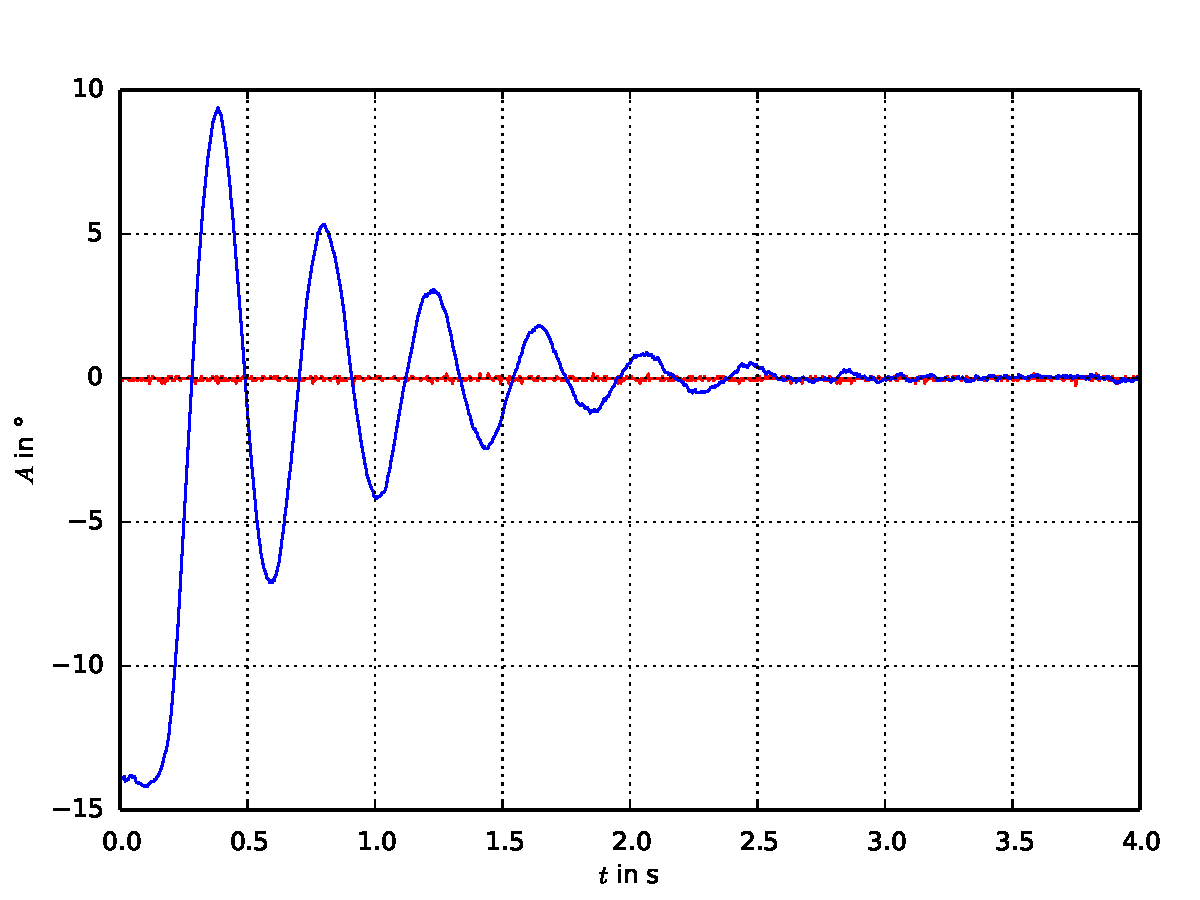
\includegraphics[width=\textwidth]{ausschwingen.pdf}
\caption{Ermitteln der Einschwingzeit}
\label{fig:plot-ausschwingen}
\end{figure}

\section{Durchführung}
Zu Beginn des Versuchs werden zusätzlich zu der Resonanz und der Kennkreisfrequenz noch acht weitere Messpunkte festgelegt und die Einschwingzeit ermittelt.
Dazu wird die Schwungmasse mit der Hand ausgelenkt und die Zeit bis zum Stillstand auf dem Oszilloskop abgelesen (vgl. \textbf{Abbildung~\ref{fig:plot-ausschwingen}})
Wichtig ist nun, dass während des Versuchs, erst nach dieser, ermittelten Einschwingzeit, die Werte auf dem Oszilloskop abgelesen werden, also das System sich im
eingeschwungenen Zustand befindet.

Nun wird das Einstellrad für die Drehzahl des Gleichstrommotors auf null gedreht und der Gleichstrommotor eingeschaltet. Anschließend wird zur
Ermittlung der Resonanzfrequenz, das Einstellrädchen langsam in Richtung steigender Drehzahl gedreht, bis die maximale Amplitude erreicht wird, welche auf
dem Oszilloskop abgelesen werden kann. Zur Ermittlung der Kennkreisfrequenz wird ähnlich vorgegangen: Experimentell wird jene Drehzahl gesucht, bei welcher
zwischen Eingangs- und Ausgangssignal ein Phasenverschub von  \SI{90}{\degree} besteht, dargestellt in \textbf{Abbildung~\ref{fig:plot-kennkreis}}.

Wurden diese beiden Winkelgeschwindigkeiten ermittelt, so werden nun nacheinander die unterschiedlichen, vorher festgelegten, Frequenzen eingestellt und
anschließend die Amplitude und die Periodendauer auf dem Oszilloskop abgelesen. Aus der Periodendauer wird die reale Winkelgeschwindigkeit errechent $\omega_{real} = \frac{2\pi}{T}$,
welche durch Ungenauigkeiten in der manuellen Einstellung von dem geplanten Wert abweichen kann. Eine Momentaufnahme zur späteren Auswertung wird gespeichert.

\begin{figure}[h]
\centering
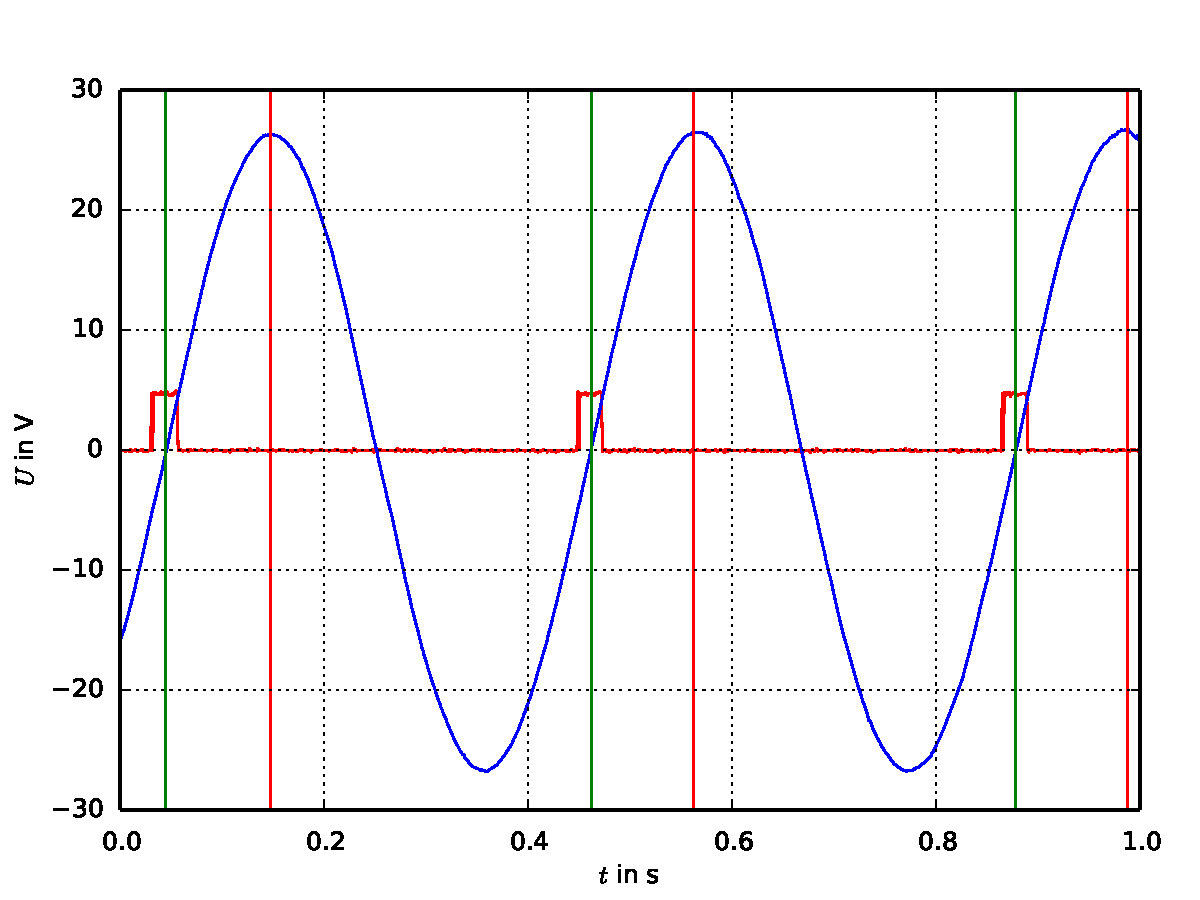
\includegraphics[width=\textwidth]{kennkreis.pdf}
\caption{Messdatenschrieb bei Kennkreisfrequenz $\omega_{n}$}
\label{fig:plot-kennkreis}
\end{figure}

\section{Auswertung}

\subsection{Rekonstruktion des Eingangssignal aus den Messungen}

Zunächst wird der Zusammenhang zwischen den tatsächlichen Zeitverläufen des Auslenkungswinkels $\alpha \left( t \right)$ und dem gemessenen Eingangssignal hergestellt.

Der Auslenkungswinkel $\alpha \left( t \right)$ des Antriebshebels verändert seine Maximalauslenkung $\gamma$ während des Versuchs nicht, jedoch wird die Drehzahl beeinflusst.
Demzufolge ändert sich die Winkelgeschwindigkeit bzw. die Zeit die benötigt wird um den Winkel $\gamma$ zu überstreichen.
Das Eingangssignal kann als ideale Sinusschwingung angenommen werden.
Es wird folglich die Periodendauer verändert. Die daraus entstehenden veränderlichen Zeitverläufe des Auslenkungswinkels $\alpha \left( t \right)$ sollen gemessen werden.

%Dies geschieht über einen Impulsgeber, welcher immer dann einen Impuls abgibt, wenn der Antriebshebel die maximale Auslenkung erreicht hat.
Dies geschieht über einen Impulsgeber, welcher einen Impuls abgibt sobald der Hebel vorbeistreicht.
Da dieser Impulsgeber sehr nah am oberen Totpunkt des Hebels montiert ist, gibt es dadurch jede Periode zwei direkt aufeinander folgende Pulse.
Wird der Mittelwert der Zeitpunkte dieser Pulse gebildet, lässt sich so unter Annahme einer konstanten Winkelgeschwindigkeit der Zeitpunkt der maximalen Amplitude des Eingangssignals ermitteln.
Das gemessene Eingangssignal gibt lediglich Aussage über die Periodendauer der Sinusschwingung nicht über dessen Amplitude.


Nun wird der maximale Auslenkungswinkel $\gamma$ berechnet. Es wird angenommen, dass die Bewegung des Antriebshebels linear verläuft und nicht als Kreisbogen.
Die gesammte Strecke, die vom Antriebshebel abgefahren wird, ergibt sich zu $2 \cdot r_1$. Nun kann der Winkel $\gamma$ errechnet werden.
\begin{equation}
	\frac{\gamma}{2} = \arcsin{\frac{r_1}{r_2}} = \arcsin{\frac{0.043}{0.235}} =  \SI{10.54}{\degree}
\end{equation}

Der insgesamt vom Antriebshebel überstrichene Winkel $\gamma$ ergibt sich somit zu $\SI{21.086}{\degree}$

\subsection{Auswertung der Ergebnisse im Bode-Diagramm}

Aus den Messschrieben des Oszilloskops lassen sich für jeden Betriebspunkt Amplitude und Phasenverschiebung des Federpendels ermitteln.
Zur Darstellung in einem Bode-Diagramm muss die Amplitude jedoch noch normiert und in die logarithmische Einheit Dezibel~(\si{\decibel}) umgerechnet werden:
\begin{equation}
	A_{\si{\decibel}} = \left.\frac{A_{aus}}{A_{ein}}\right\rvert_{\si{\decibel}}
		= \left.\frac{A_{aus}}{\SI{10.54}{\degree}}\right\rvert_{\si{\decibel}}
		= \left.A_{rel}\right\rvert_{\si{\decibel}}
		= 20 \cdot 10^{A_{rel}} \, \si{\decibel}
\end{equation}

Zur Glättung der Messwerte wurde ein exponentiell gewichteter laufender Mittelwert verwendet, wobei das Verfahren zur Korrektur einer dabei auftretenden Phasenverschiebung einmal vorwärts und einmal rückwärts angewendet wurde, \cite{ewma}.

In \textbf{Tabelle~\ref{tab:messwerte}} sind die ermittelten Messdaten zusammengestellt.
\begin{table}[h]
	\centering
	\caption{Messwerte}
	\label{tab:messwerte}
	\begin{tabular}{lrrrr}
	\toprule
	geplant           & $\omega$&     $A$ &   $A_{\si{\decibel}}$ & $\Delta \varphi$ \\
	  & \si{\radian\per\second} & \si{\degree} & \si{\decibel} & \si{\degree} \\
	\midrule
	$\omega_n$        &  15.09 &  53.66 &  14.14 &  -86.5 \\
	$\omega_r$        &  15.06 &  50.30 &  13.57 &  -82.9 \\
	\SI{0.5}{\hertz}  &   3.36 &   9.93 &  -0.52 &   -2.3 \\
	\SI{0.7}{\hertz}  &   4.70 &  10.28 &  -0.22 &    1.1 \\
	\SI{1.0}{\hertz}  &   6.71 &  11.37 &   0.65 &   -4.6 \\
	\SI{1.3}{\hertz}  &   8.56 &  13.60 &   2.22 &   -8.8 \\
	\SI{1.5}{\hertz}  &   9.86 &  16.17 &   3.72 &  -10.2 \\
	\SI{2.0}{\hertz}  &  12.91 &  31.23 &   9.44 &  -23.7 \\
	\SI{2.5}{\hertz}  &  15.85 &  43.37 &  12.29 & -120.0 \\
	\SI{3.0}{\hertz}  &  18.81 &  14.99 &   3.06 & -155.2 \\
	\SI{4.0}{\hertz}  &  24.71 &   5.65 &  -5.42 & -160.2 \\
	\SI{5.0}{\hertz}  &  30.69 &   2.92 & -11.14 & -168.6 \\
	\bottomrule
	\end{tabular}
\end{table}

Trägt man in einem Diagramm mit logarithmischer x-Achse die logarithmische normierte Amplitude $A_{\si{\decibel}}$ sowie die Phasenverschiebung $\Delta \varphi$ über der Kreisfrequenz $\omega$ auf erhält man ein Bode-Diagramm, dargestellt in \textbf{Abbildung~\ref{fig:plot-bode}}.
\begin{figure}[h]
\centering
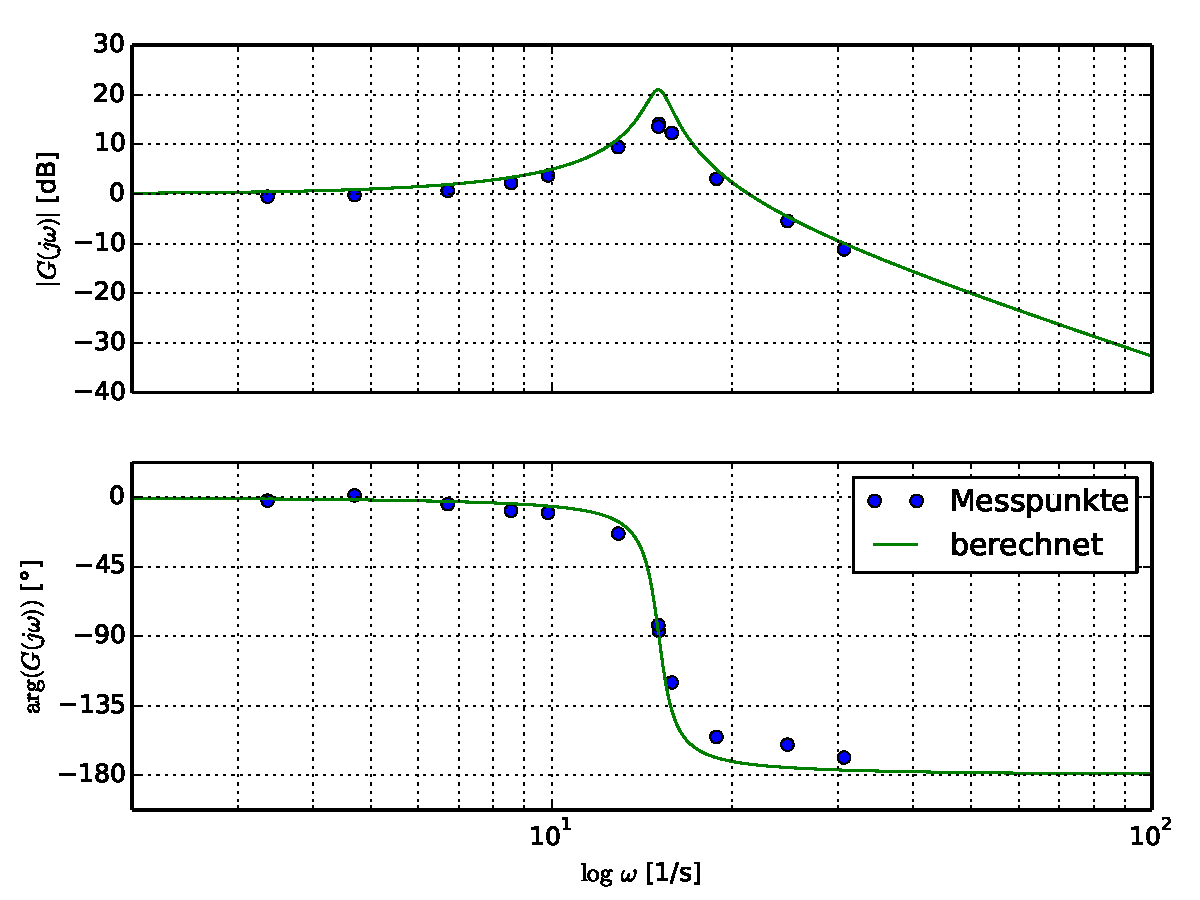
\includegraphics[width=\textwidth]{bode.pdf}
\caption{Bode-Diagramm}
\label{fig:plot-bode}
\end{figure}

\subsection{Identifikation der Systemparameter} % ich habe jetzt einfach nur die Berechnung des Trägheitsmoments eingebaut...

Um das Trägheitsmoment der Aluminiumscheibe zu berechnen, sehen wir diese als Zylinder an.
Nach \cite{tbmetall}  gilt:
\begin{equation}
	\label{eq:J}
	J_z = \frac{1}{2} \cdot M \cdot R^2
\end{equation}

Mit eingesetzten Werten ergibt sich somit:
\begin{gather}
	R = \SI{0.2}{\metre} \\
	h = \SI{9.4e-3}{\metre} \\
	\rho = \SI{2.7e6}{\gram\per\cubic\metre}
\end{gather}
\begin{align}
	M &= \rho \cdot \pi \cdot R^2 \cdot h \\
	&= \SI{2.7e6}{\gram\per\cubic\metre} \cdot \pi \cdot \left( \SI{0.2}{\metre} \right)^2 \cdot \SI{9.4e-3}{\metre} \\
	&= \SI{3.189}{\kilogram}
\end{align}

Eingesetzt in (\ref{eq:J}) erhält man für das Trägheitsmoment $J_{z}$:
\begin{equation}
	J_z = \frac{1}{2} \cdot \SI{3.189}{\kilogram} \cdot {\SI{0.2}{\metre}}^2 = \SI{63.79e-3}{\kilogram\square\metre}
\end{equation}

%Somit ergibt sich das Trägheitsmoment der Aluminiumscheibe zu $\SI{0.06}{\kilogram\square\metre}$
Das Trägheitsmoment der Aluminiumscheibe beträgt somitt $J_{z} = \SI{63.79e-3}{\kilogram\square\metre}$.

Nach \cite{skript} gilt:
\begin{equation}
	\label{eq:D}
	D = \sqrt{ \frac{1 - \left( \frac{\omega_{r}}{\omega_{n}} \right)^{2}}{2} }
		= \sqrt{ \frac{1 - \left( \frac{\SI{15.06}{\radian\per\second}}{\SI{15.09}{\radian\per\second}} \right)^{2}}{2} }
%		= \sqrt{ \frac{1 - \left( 0.998 \right)^{2}}{2} }
%		= \sqrt{ \frac{\num{3.973e-3}}{2} }
		= \num{44.57e3}
\end{equation}

Setzt man die experimentell ermittelten Werte für die Kennkreisfrequenz $\omega_{n}$ und die Resonanzfrequenz $\omega_{n}$ ein (\textbf{Tabelle~\ref{tab:messwerte}}), ergibt sich eine Dämpfung von $D = 0.045$, vgl.~(\ref{eq:D}). Beim Vergleich des Bode-Diagramms mit Abbildungen in der Literatur erscheint dieser Wert plausibel.

Setzt man die Dämpfung und die Kennkreisfrequenz in die Übertragungsfunktion eines PT2s-Systems mit einer stationären Verstärkung von $K_{P} = 1$ ein, erhält man die Übertragungsfunktion des verwendeten Federpendels im Bildbereich:
\begin{equation}
	\label{eq:Gs}
	G \left( s \right) = \frac{K_{P}}{\frac{1}{\omega_{n}^{2}} s^{2} + \frac{2 D}{\omega_{n}} s + 1} = \frac{1}{0.00439 s^{2} + 0.00591 s + 1}
\end{equation}

In \textbf{Abbildung~\ref{fig:plot-bode}} ist neben den Messpunkten ebenfalls der Frequenzgang der in (\ref{eq:Gs}) ermittelten Übertragungsfunktion dargestellt.
Es ist ersichtlich, dass das System in Wirklichkeit stärker gedämpft ist als das aufgestellte Modell zeigt. \todo{Sebastian: warum?}

Aus \cite{skript} ist bekannt:
\begin{gather}
	\frac{1}{\omega_{n}^{2}} = \frac{k}{J} \\
	\frac{2 D}{\omega_{n}} = \frac{d}{k}
\end{gather}

Umgestellt und eingesetzt ergibt sich: \todo{ist das plausibel?}
\begin{gather}
	k = J \cdot \omega_{n}^{2} = \SI{63.79e-3}{\kilogram\square\metre} \cdot \left( \SI{15.09}{\radian\per\second} \right)^{2} = \SI{14.52e3}{\newton\metre\per\radian}\\
	d = \frac{2 \cdot D \cdot k}{\omega_{n}} = \SI{85.78}{\newton\metre\second\per\radian}
\end{gather}

\section{Fehlerbetrachtung}
Hinsichtlich der Erfassung und Protokollierung der Messwerte der
Frequenzganganalyse können verschiedene Fehler auftreten. Die verschiedenen Fehler
sind in systematische, stochastische und methodische Fehler zu unterschieden.
Systematische Fehler sind bei identischer Anwendung reproduzierbar und sofern diese
bekannt sind, auch korrigierbar. Ein systematischer Fehler wäre bei diesem Versuch
zum Beispiel, dass die Eingangsschwingung keine ideale Sinusschwingung aufgrund
des Kurbelbetriebs aufweist. Ferner ist die Federkonstante von der Temp eratur
abhängig, was eine weiter Fehlerquelle aufzeigt. Die Temperatur wird nicht gemessen
und somit können auch die Reibungsverluste die in den Lager auftreten nicht
berücksichtigt werden. Der Elektromotor läuft bei niedrigen Drehzahlen unruhig und
es sind Toleranzabweichungen in den Messgeräten vorhanden. Stochastische Fehler
können bei diesem Versuch in verschiedenen Arten vorkommen. Einerseits kann ein
Messrauschen, wie es aus der Messtechnik und Signalübertragung bekannt ist, die
angezeigten Ergebnisse verfälschen, andererseits können auch menschliche Fehler
entstehen. Hier ist vor allen der Ablesefehler zu nennen. Auch Rundungsfehler sind
in den Berechnungen zu berücksichtigen. Insbesondere durch das glätten der
aufgezeichneten Messwerte. Diese Fehler lassen sich in der Regel nur schwer
korrigieren und auch vermeiden. Ein methodischer Fehler liegt in dem Versuch durch
die geringe Anzahl der Messpunkte von insgesamt einem Dutzend vor, dadurch lässt sich
ein vollständiges Bodediagramm nicht abbilden.

\section{Fazit}
Dieser Versuch hat gezeigt, dass es möglich ist den Frequenzgang von Systemen experimentell zu bestimmen und so Aufschluss über das Verhalten
bei bestimmten Frequenzen zu bekommen. Dies ist für viele schwingende Bauteile relevant, da die Amplitude stark variieren kann und somit auch
der Verschleiß. Es ist also zum Beispiel interessant das Verhalten eines Bauteils so anzupassen, dass die Resonanzfrequenz und somit auch die
überhöhte Amplitude im Betrieb vermieden wird. Dazu wurden hier im Versuch verschiedene, auf den Frequenzgang Einfluss nehmende Größen bestimmt.
Wenn man den genauen Zusammenhang dieser Größen im Bauteil versteht, so kann man einzelne von ihnen ändern und so durch relativ leichte eingriffe
starken Einfluss auf das Schwingverhalten und somit auch die Betriebsfestigkeit nehmen.


\pagebreak
\nocite{*}
\sloppy % großzügige Wortabstände zulassen --> URLs werden umgebrochen
\printbibliography


\end{document}

